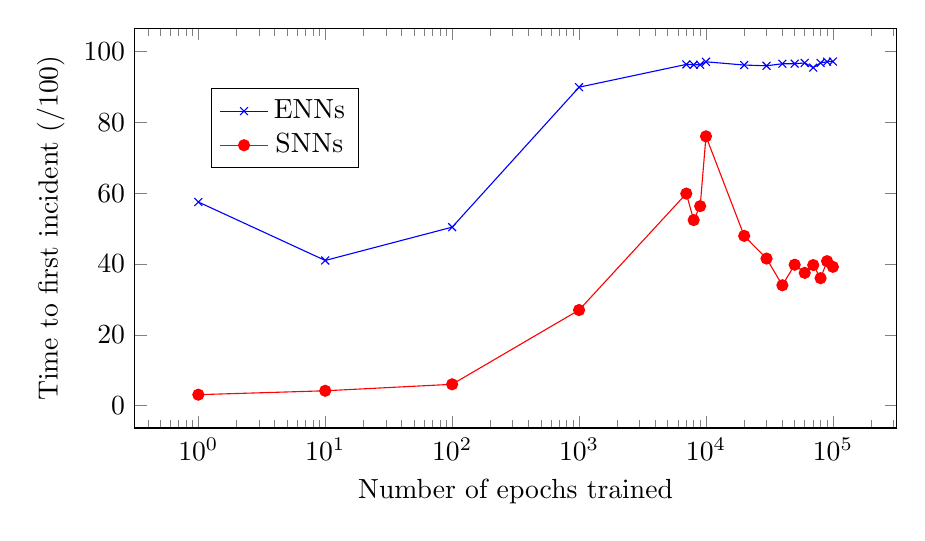
\begin{tikzpicture}
\begin{semilogxaxis}[
xlabel={Number of epochs trained},
ylabel={Time to first incident (/100)},
x=0.7cm,
y=0.45mm, 
legend style={at={(0.1,0.75)},anchor=west}]

\addplot[color=blue,mark=x] coordinates {
	(0, 52.5)
	(1, 57.5)
	(10, 41.0)
	(100, 50.4)
	(1000, 89.9)
	(7000, 96.33)
	(8000, 96.21)
	(9000, 96.24)
	(10000, 97.07)
	(20000, 96.15)
	(30000, 95.94)
	(40000, 96.52)
	(50000, 96.53)
	(60000, 96.74)
	(70000, 95.44)
	(80000, 96.75)
	(90000, 97.09)
	(100000, 97.14)
};


\addplot[color=red,mark=*] coordinates {
	(0, 2.95)
	(1, 3.12)
	(10, 4.22)
	(100, 6.05)
	(1000, 27.01)
	(7000, 59.87)
	(8000, 52.39)
	(9000, 56.33)
	(10000, 76.03)
	(20000, 47.94)
	(30000, 41.54)
	(40000, 34)
	(50000, 39.8)
	(60000, 37.5)
	(70000, 39.7)
	(80000, 36)
	(90000, 40.8)
	(100000, 39.2)
};


\legend{ENNs, SNNs}
\end{semilogxaxis}%
\end{tikzpicture}%